We have split our firmware into a number of separate modules, as shown in figure
\ref{fig:fw_block_diag}. All of the drivers for microcontroller peripherals
such as serial interfaces and the ADC are provided by the nRF52 SDK, which is a
library provided by Nordic Semiconductor, the manufacturer of the nRF52840
microcontroller we are using. We are also using some higher level components
from the nRF52 SDK such as the USB CDC-ACM stack, a FAT32 filesystem driver and
Nordic's soft device S140 which is a Bluetooth LE peripheral stack.

These third party components will be used by the software we wrote ourselves
which includes the drivers for all of our sensors (IMU, optical heart rate
sensor, air quality sensor and UV light sensor) as well as the signal processing
code required to derive a heart rate from the raw data we receive from our
optical heart rate sensor. While we plan to use a third party file system
implementation we will still need to write the code that allows blocks to be
written to and read from an SD card over an SPI interface.

At the application layer we have three modules. Our data logging service is
responsible for most of the operation of our device and continually collects
and logs sensor data. The Bluetooth data transfer service facilitates accessing
the logged data over a Bluetooth interface. Our debugging interface exposes our
firmware functionality over a USB serial interface so that integration tests can
be run on the microcontroller.

\begin{figure}[!htb]
\centering
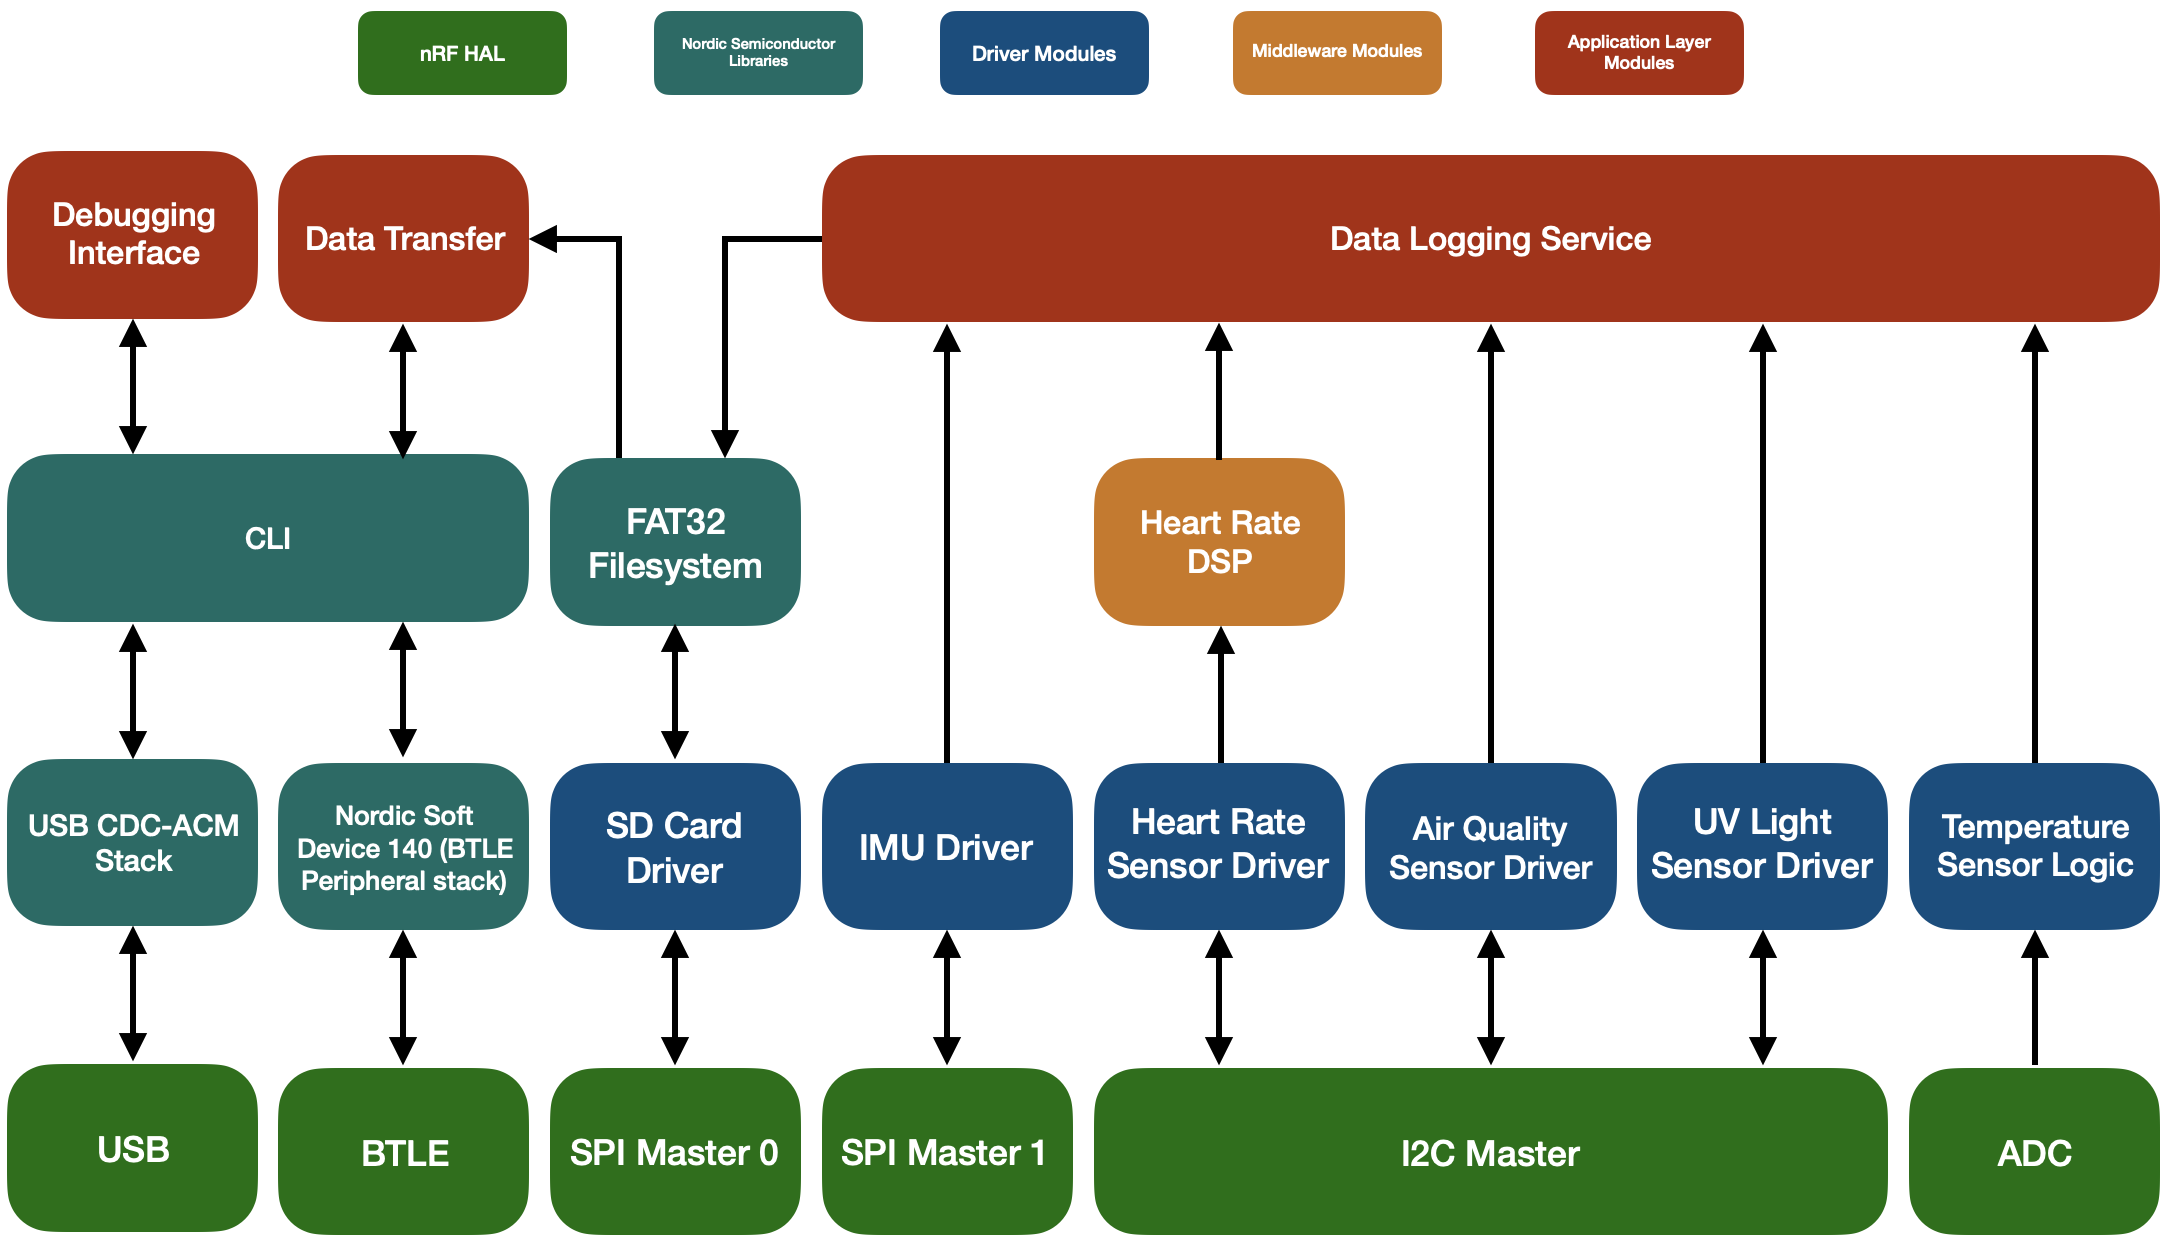
\includegraphics[width=\textwidth]{images/fw_block_diag.png}
\caption{Firmware block diagram.}
\label{fig:fw_block_diag}
\end{figure}

\subsection{Super Loop}

We chose to use a super loop architecture for our firmware because we predicted
that the approach would be sufficient for our needs and would be easier for us
to implement then making use of a realtime operating system. Our firmware
consists of an initialization section followed by an infinite main loop.

Our code is separated in to a number of software modules (as shown in figure
\ref{fig:fw_block_diag}). The software modules that we wrote have an
initialization function which is called once on system startup. Some of our
firmware module are entirely interrupt based, but many have a service function
which is run in each iteration of the main loop.

Figure \ref{fig:fw_flow} shows the flow of our firmware. We start with a number
of initialization tasks before starting to loop through the service functions
for our modules. Each service function will check if there is any work to be
done for a specific module and start and tasks that are ready to begin. After
each iteration of the main loop the wait for interrupt instruction is used to
cause the processor to enter a sleep mode until an interrupt occurs. We have a
timer configured to generate interrupts every millisecond to increment a count
which is used as a time reference throughout the firmware, because of this the
processor will sleep for at most one millisecond at a time.

\begin{figure}[!htb]
\centering
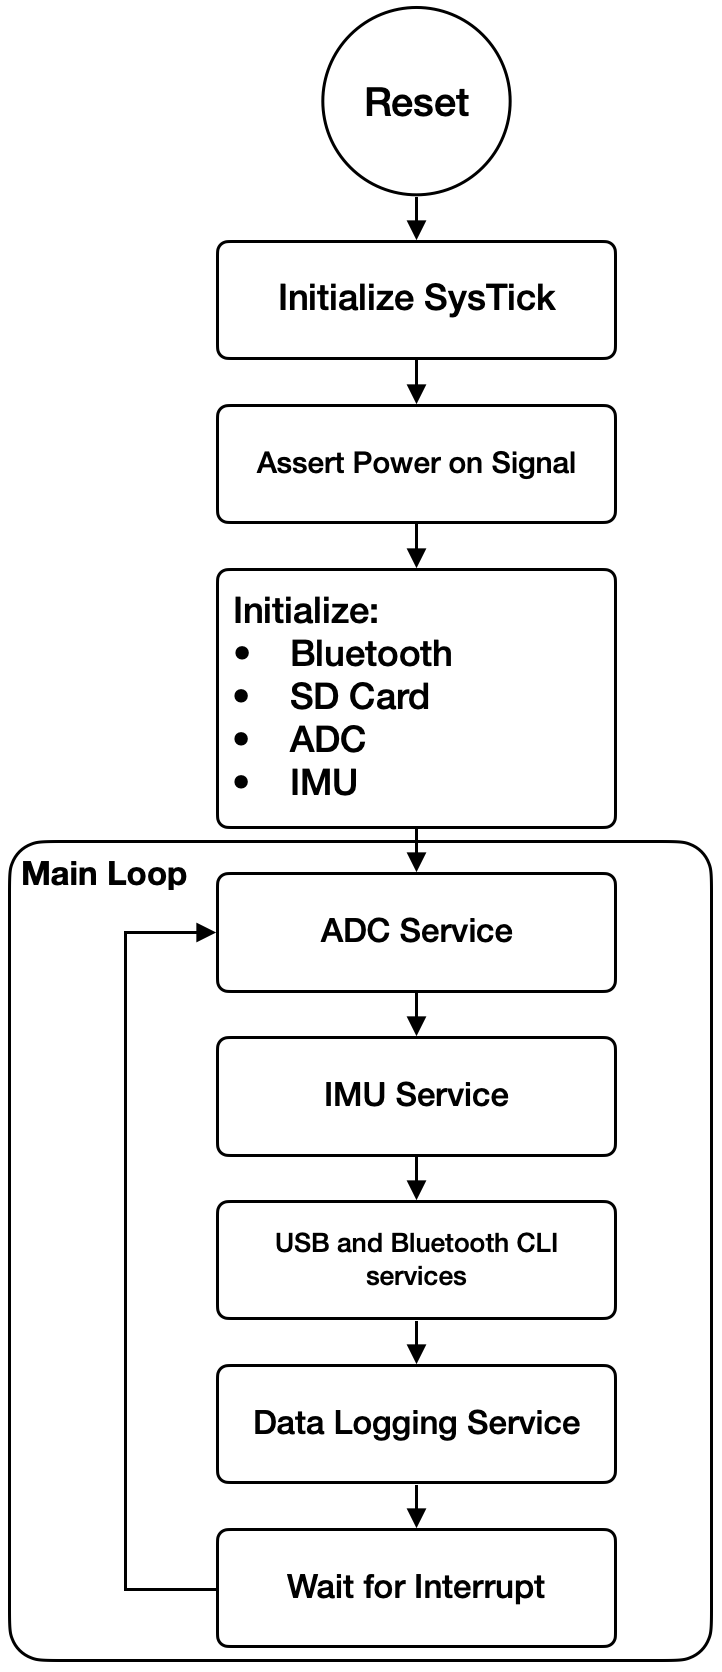
\includegraphics[width=0.4\textwidth]{images/fw_flow.png}
\caption{Firmware flow chart.}
\label{fig:fw_flow}
\end{figure}

The super loop architecture is a cooperative multitasking system. This makes it
important that the service function which are called in the main loop do not
block for long periods. If a service function was to block it would prevent the
other software modules on the system from operating correctly. In order to meet
this requirement our service functions are written as state machines. Modules
keep track of their current state and are able to determine what, if anything,
needs to be done in each iteration of the main loop based on their state.

We were not able to completely avoid blocking in the main loop because of our
use of a third party FAT filesystem implementation. The filesystem implementation
blocks while writing to the SD card. The performance implication of this are
discussed in section \ref{subsec:testing-data-logging}.

\subsection{Interrupts and Bluetooth Soft Device}

Our firmware makes use of a bluetooth stack provided by Nordic Semiconductor
know as the S140 Soft Device. This "soft device" is distributed as a binary
blob which is flashed to the microcontroller separately from the application
software. The soft device takes ownership of number of microcontroller
peripherals including the radio hardware, clock and power management peripherals,
multiple timers, non-volatile memory controller and cryptography accelerators.
The soft device schedules itself independently of the application using on of
the microcontroller's real time clocks and application software interacts with
the soft device using supervisor calls.

All interrupts are received by a piece of code called the master boot record
(MBR). The MBR then forwards them to the soft device if there is one installed
on the microcontroller. The soft device uses some interrupts for its own
purposes, interrupts which the soft device does not use are forwarded to the
application. Nordic Semiconductor specifies that this forwarding process adds
less than three microseconds of latency to peripheral interrupts which are to
handled by the application.

Figure \ref{fig:fw_int_prio} shows the interrupt priorities used in our system.
The priority levels shown in red are reserved by the soft device bluetooth
stack, those shown in blue are available for use by application software. The
soft device uses the highest interrupt priority level for its timing critical
interrupts. The second highest interrupt priority level is reserved for the
soft device's peripheral access control fault handler so that the soft device
can safely handle any faults which are caused by application interrupts. The
soft device also used priority level four for API calls and processing tasks
that are not time critical.

\begin{figure}[!htb]
\centering
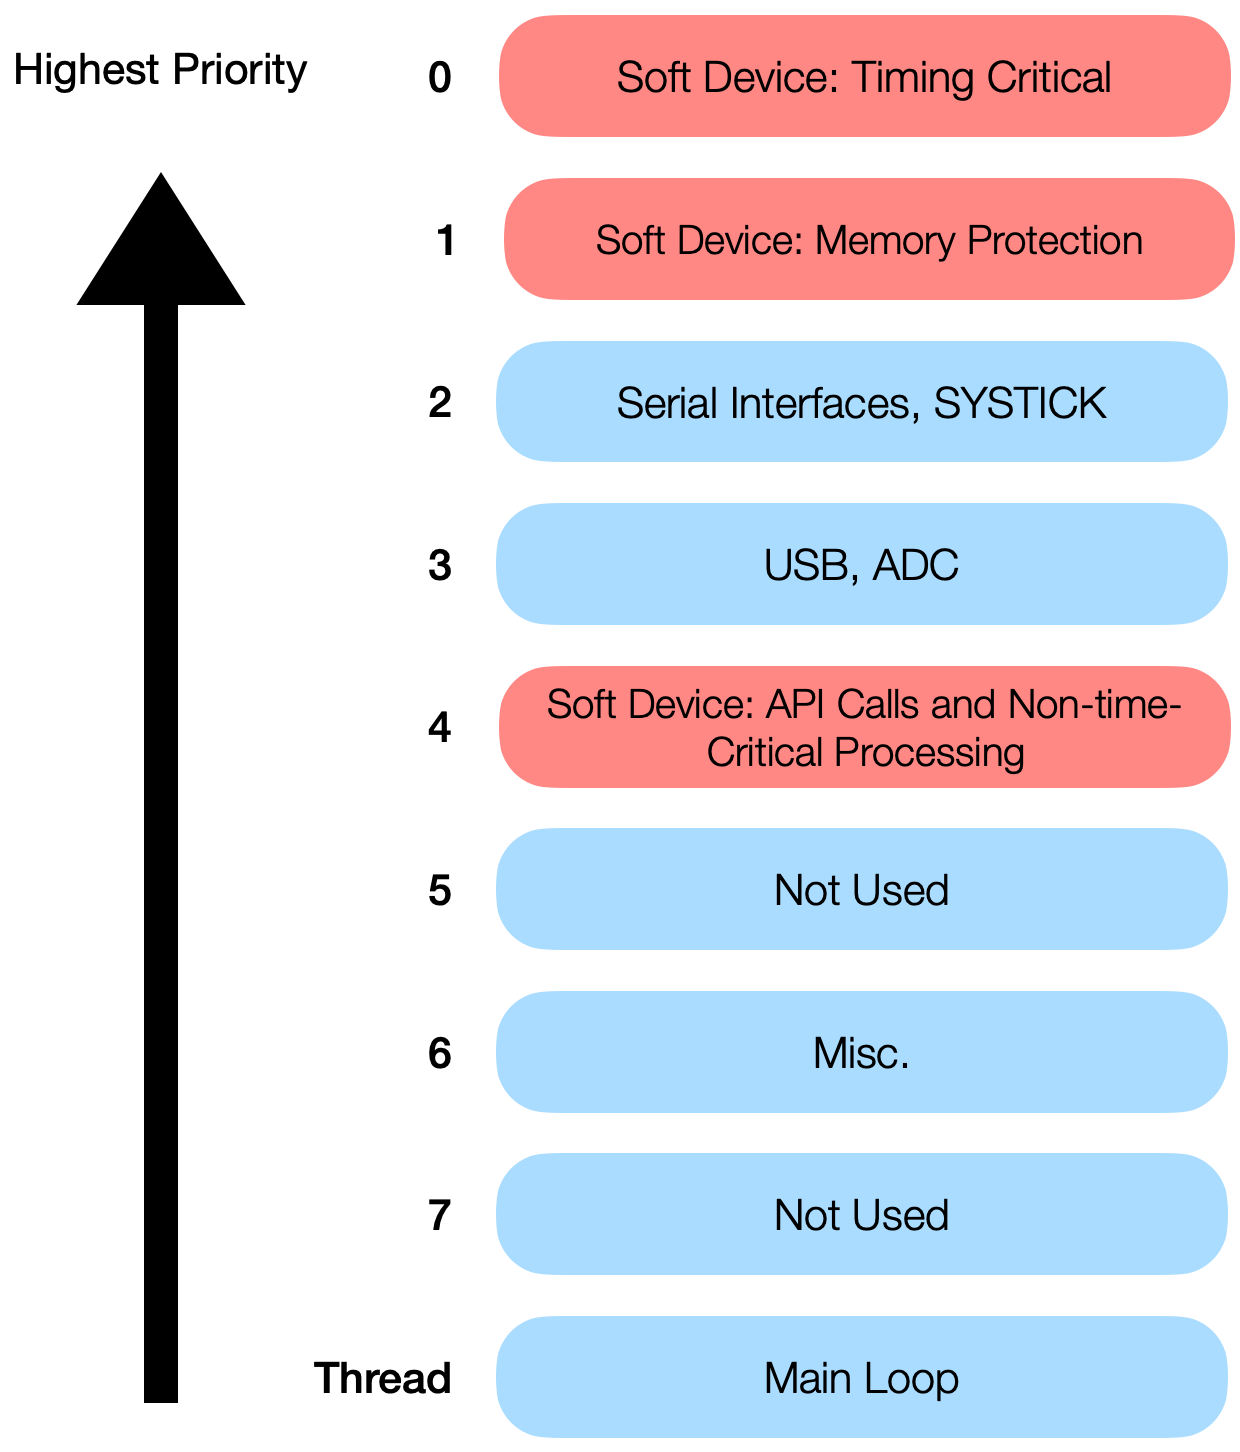
\includegraphics[width=0.5\textwidth]{images/fw_int_prio.png}
\caption{Interrupt priorities.}
\label{fig:fw_int_prio}
\end{figure}

Most of our application interrupts are configure at priority levels two and
three. Our interrupts are grouped into SysTick and and serial interface
interrupts at priority two and USB and ADC interrupts at priority three.

The priority two interrupts are those which we expect to be very short. The
SysTick interrupt is at a high priority to avoid help avoid hitter in our system
time and the serial interrupts are placed at priority two to achieve the best
possible serial interface performance.

\subsection{Data Logging}

The core of our firmware is the data logging service. Sensor drivers push data
to this software module which is buffered and then later stored to the SD card
using the FAT filesystem. The data logging module has two 512 byte buffers. The
module fills one buffer, then writes it to the SD card as it begins to fill the
other.

Figure \ref{fig:fw_data_flow} illustrates the flow of data through the data
logging service. Each sensor driver pushes data to the data logging service at a
rate selected based on the type of data that the sensor produces. Every sample
of sensor data is wrapped in a header that indicates the current system time
when the value was collected, the type of data and the length of the data and
the resulting packet is added to the data logging service buffer. Approximately
once per second the data logging buffer will be written to the SD card using the
filesystem driver.

\begin{figure}[!htb]
\centering
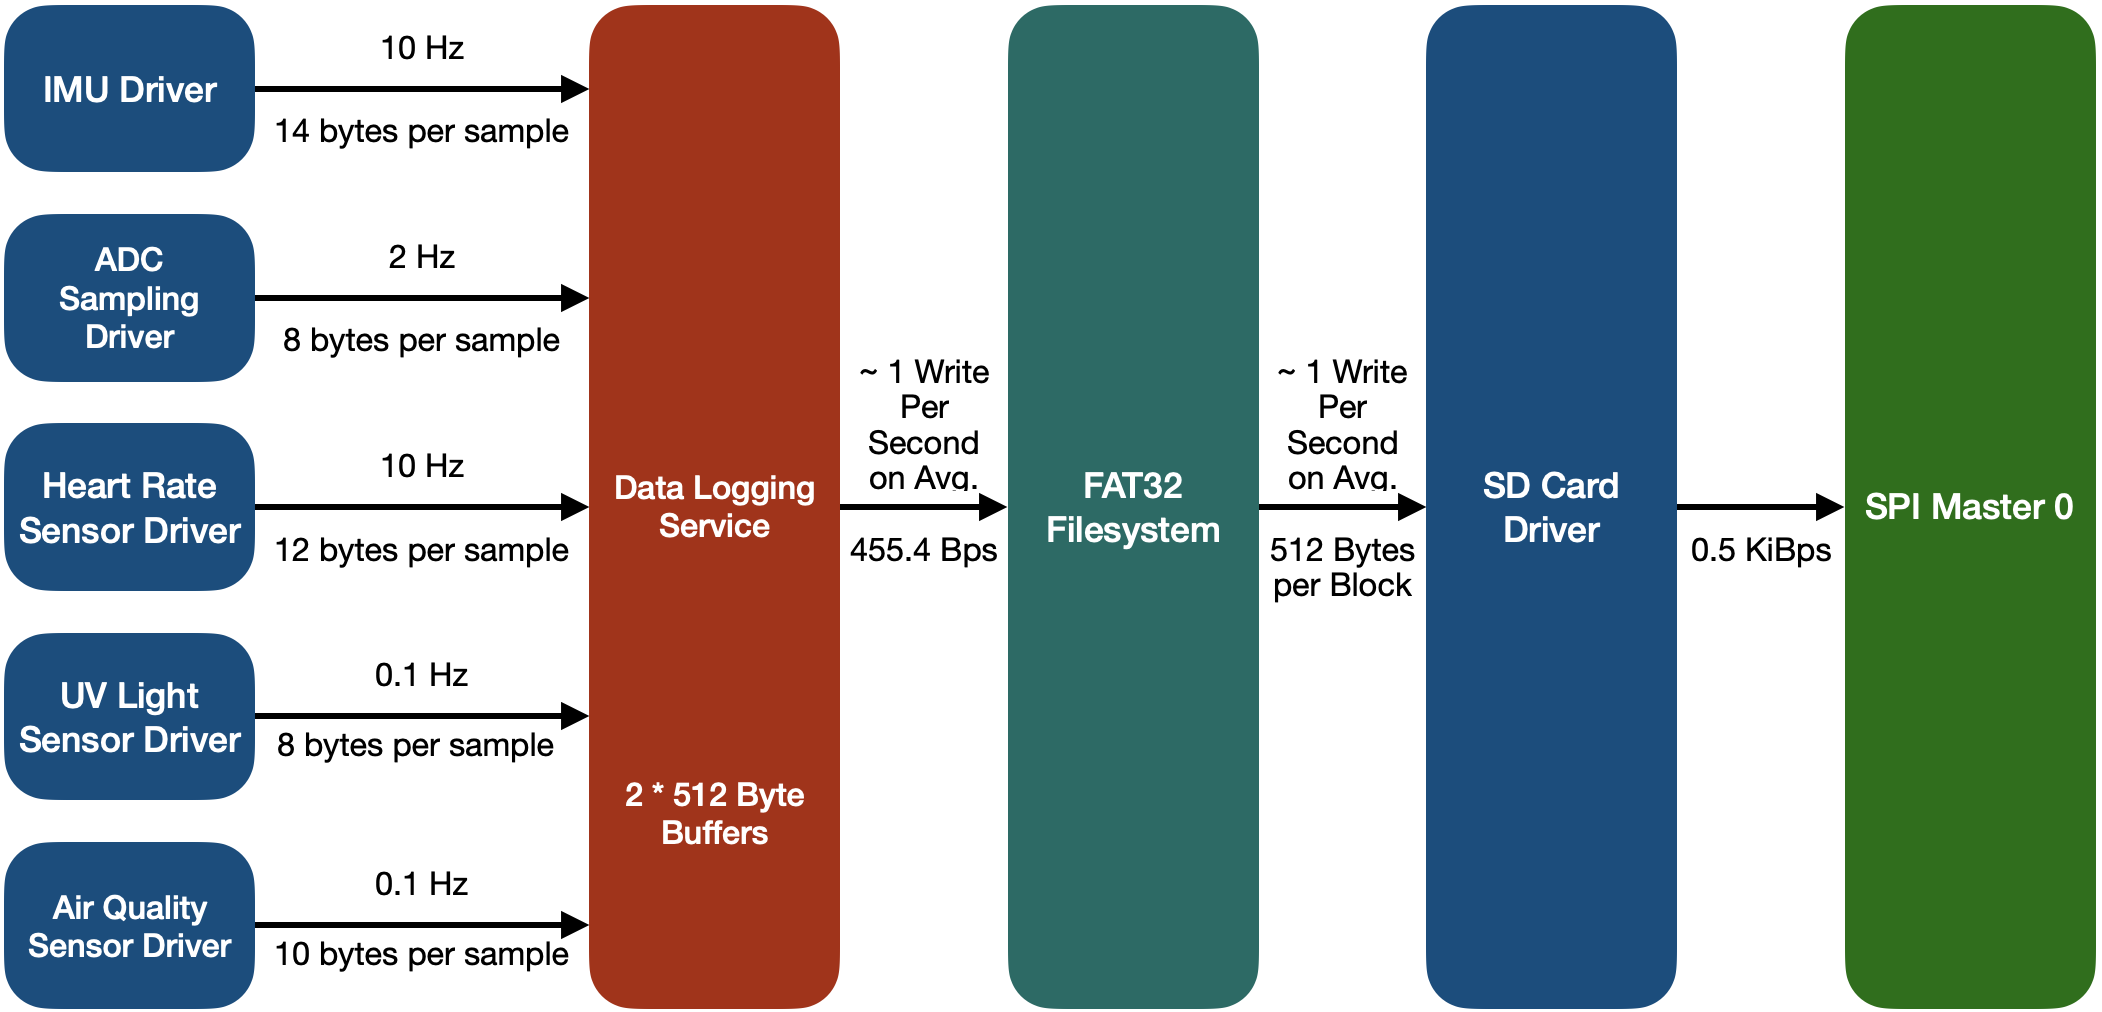
\includegraphics[width=\textwidth]{images/fw_data_flow.png}
\caption{Data flow.}
\label{fig:fw_data_flow}
\end{figure}

\subsection{Drivers}

\subsubsection{USB}

The USB serial interface software module provides a simple abstraction over the
nRF5 SDK's USB communications device class abstract communications model
(CDC-ACM) driver which allows for serial port emulation. The USB serial module
maintains circular buffers for input and output and provides a variety of
functions for reading from and writing to the buffers. The output buffer can be
written to in a blocking or non-blocking fashion. The input buffer can be read
character by character, in blocks, or by line with a selectable delimiter.

\subsubsection{Bluetooth}

The design goal for the Bluetooth driver was to have it behave like a serial
port in the same fashion that USB CDC does. Our intention in doing this was to 
simplify the design of the companion software as well as the command line 
interface present on the microcontroller. This goal was fully achieved 
on the microcontroller side of the communication link. The software interface for 
Bluetooth was made identical to USB so that they can be used interchangeably 
without additional complications. On the PC side where the companion software
runs the solution was not as elegant. We had hoped to find a way to make the
Bluetooth connection appear as a serial port so it could be used interchangeably
with the USB CDC connection, but a method to do this was not found. It likely
could be done by writing custom drivers, but this was outside the scope of the
project. Instead, a cross platform Python library was used to establish the
Bluetooth connection to the device and communicate with it as you normally
would with a Bluetooth device.

The device uses Bluetooth Low Energy, which works by advertising
available services to other nearby devices. Each service may offer a number
of characteristics that can be read only, write only, read-write, and have 
several other options such as notifying a connected device when a characteristic
value changes. The Bluetooth Low Energy specification includes descriptions of several
standard services and their characteristics, but none of these could be used to
to achieve the serial port-like behaviour needed for this project. A custom
serial port service included with the Nordic SDK was used instead. This service
has two characteristics, one named TX and one named RX. The RX characteristic is
write only and is used to send data to the device. The TX characteristic is
written to only by the device and has notifications enabled. If a connected device
wants to receive data then it must subscribe to the notifications of the TX 
characteristic. This solution worked out quite well, although it has a low 
throughput in comparison to USB. The fact that each notification packet can only 
hold approximately 20 bytes and must be acknowledged before the next one is 
sent likely contributes to the low throughput significantly. It was not expected
that Bluetooth Low Energy would be very fast however, since it is optimized for 
power consumption instead of speed. This trade-off is well suited to this project 
because it is battery powered.

\subsubsection{Heart Rate Sensor}

Our heart rate driver is based on an open source implementation written in
C++ \cite{max86150-ardino}. Since the SDK we are using falls under the nRF5
Nordic License, only software that is compatible with this license can be
integrated into the project. The open source C++ heart rate driver is under the
expat license so we are free to use it as long as the copyright notice is
maintained. Unfortunately, not all useful open source software was licensed in
a way compatible with the SDK license. In particular, it would have been ideal
to reuse an algorithm to convert raw PPG data to beats per minute, however the
available algorithm was licensed with the Lesser GNU Public
License \cite{wasp-os} which is incompatible with the SDK license.

\subsubsection{Inertial Measurement Unit}

Our driver for the ICM 20948 IMU is written from scratch. The driver is a finite
state machine that makes use of the nRF5 SDK's SPI driver. The state machine
controls the process of initializing the sensor and of periodically taking
readings, which are then handed off to the data logging service to be recorded.

A simplified state diagram for the IMU driver is shown in figure
\ref{fig:fw_imu_fsm}.

\begin{figure}[!htb]
\centering
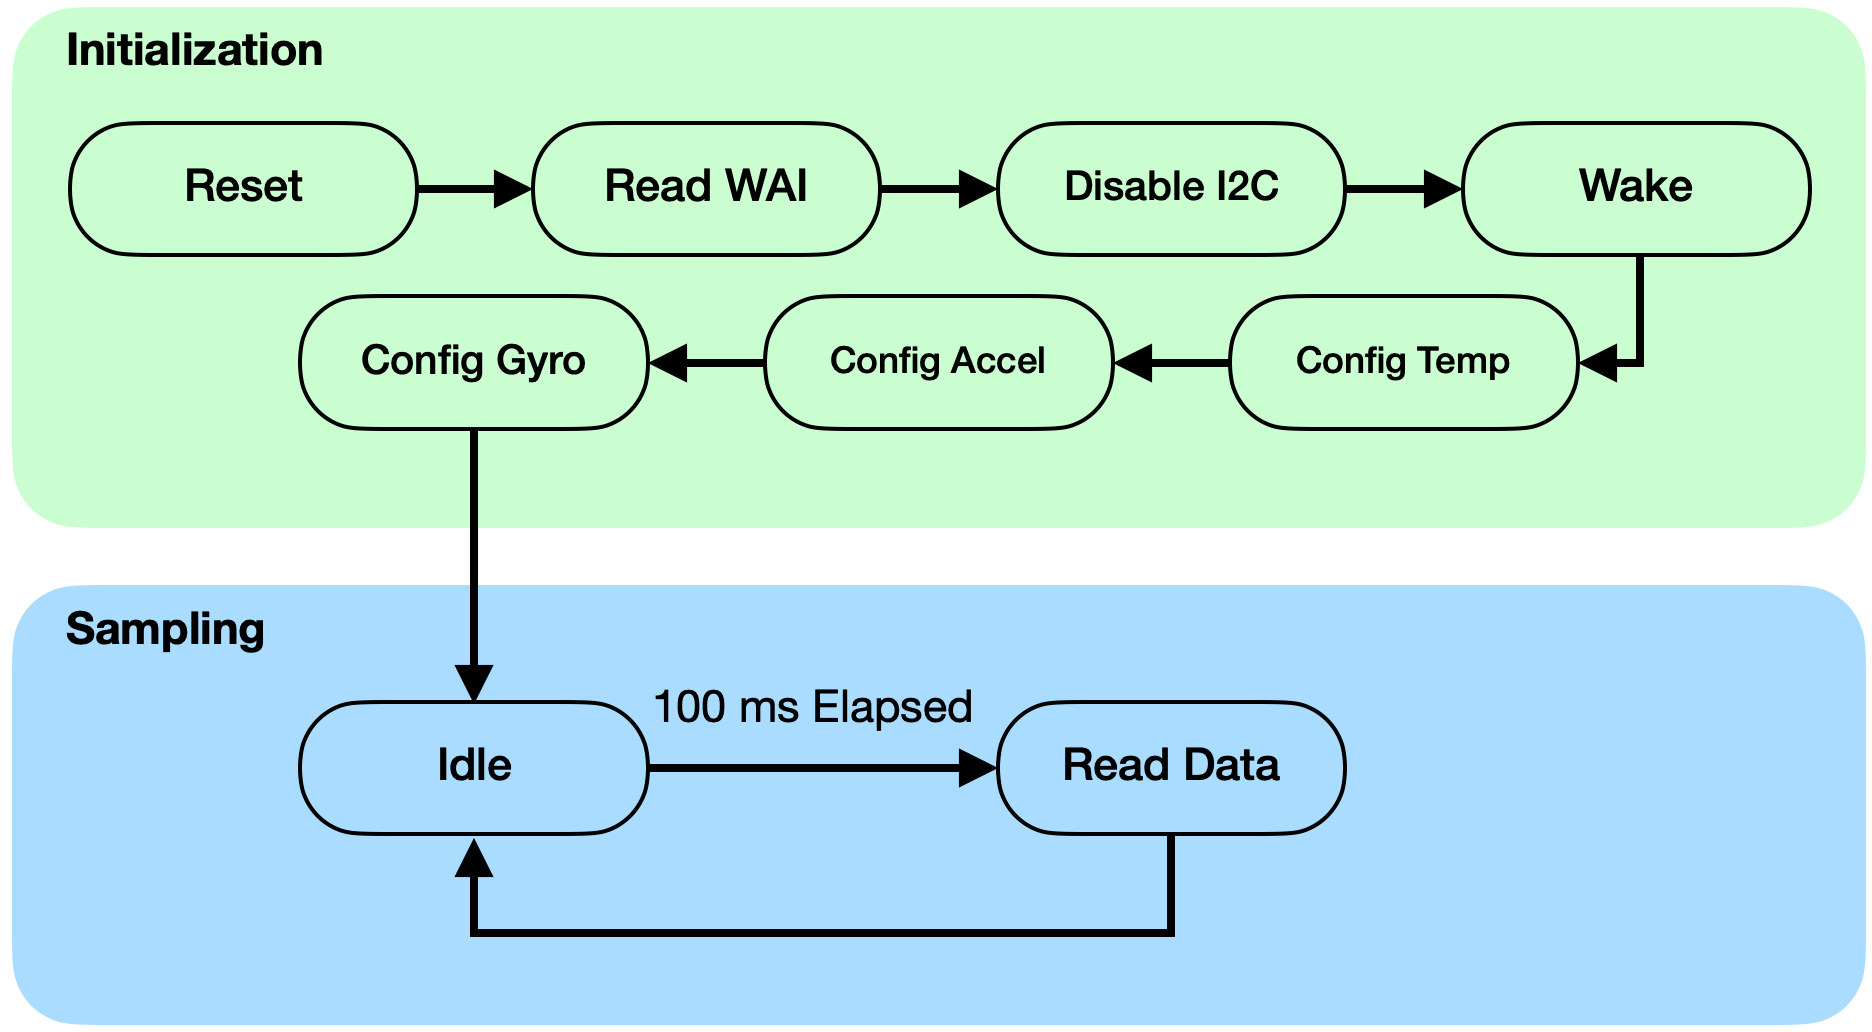
\includegraphics[width=0.8\textwidth]{images/fw_imu_fsm.png}
\caption{IMU driver state machine.}
\label{fig:fw_imu_fsm}
\end{figure}

\subsection{Command Line Interface}

Our firmware provides a command line interface (CLI) which is available via the
USB or bluetooth serial interfaces. This command line interface is used for
debugging, testing and for interaction with the companion app. Our CLI
abstraction provides an identical interface over USB or bluetooth.

The CLI provides a number of commands which are intended for human interaction
including commands for printing out sensor data, accessing profiling information,
writing test messages to the SD card and reading directories and files from the
SD card.

The CLI also has a number of commands which are intended to interact with our
companion software. These functions allow the companion software to read files
from the SD card. The files are written out over the serial interface in
hexadecimal format.

\subsection{Companion App}

The companion app is a desktop application written in python to connect to the device, extract the log data and convert it into a plain text format convenient for further analysis.

Since during development there were a number of things that were likely to change or unknown, the companion software was designed to be highly modular so that each part was isolated for sake of testing and updating.  The flow of data is described by the following flow diagram:

% TODO Flow diagram

\subsubsection{Extracting log file}

When the device is connected over USB the companion software can be run to open a serial connection with the device, otherwise the companion software will scan for the device over bluetooth and attempt to pair and connect.  Once a bluetooth connection is established a wrapper is created to emulate the same behaviour as a serial connection so that the CLI communication module can use both connections interchangeably.

The interaction with the CLI consists of sending a time alignment command and using 'hcat' command to read the offset file and log file.  

Since the device does not have time keeping all log entries are recorded with internal timestamps only, the time alignment command creates a log entry matching an internal timestamp with a unix timestamp generated by the companion app.  

The log file consists of binary data blobs with variable length so identifying the boundaries of entries from the middle of the file is impossible without additional context, for this reason a separate file is kept with a list of offsets corresponding to each reset so an option can enable only recording data from a given reset index.

\subsubsection{Parsing log file}

Once the log file is obtained either by extracting it through the CLI interface or by extracting it from the SD card directly, it is converted from a binary format into plain text CSV files for each type of entry.

The module which parses the headers will read the length of each entry's payload and ensure the correct length of bytes is being read.  Particularly if an entry is only partially written when the device loses power a reset index specified by the separate file will indicate this and the partial entry can be discarded without corrupting all subsequent data.

The module which parses the payloads relies on introspection and struct definitions for each entry type.  The order and types of the fields are used to extract data from the log file while the name of the struct defines the name of the csv file created and the variable names in the struct are used to generate a header for the csv.  This way adding a new sensor requires only adding a struct and no additional parsing code is needed.

Unit adjustment was accounted for in the original plan however since all log entries are adjusted on the device to be fixed power of 10 of a useful unit (for example accelerometer data is $10^{-4} g$ where $g$ is a standard gravity unit) the companion app doesn't do additional adjustments. 

Some additional code is used to create a graph of a selected csv file for demonstration purposes, this also can produce live updating graphs

% TODO: talk more about live updating stuff?
% what else did I miss?
